\newpage
\section{A Large Ion Collider Experiment at the LHC}

ALICE (A Large Ion Collider Experiment) is one of major experiment at LHC (Large Hadron Collider) in Geneva and it is dedicated experiment for the study of QCD matter created in high-energy collisions \cite{cite:ALICEPerformance}. It has been accumulating data during the whole first phase of the LHC operation, from end of 2009 to the beginning of the technical shutdown 2013. During that time, the beam energy was tuned to have data in pp collisions at 0.9, 2.76, 7 and 8 TeV, p--Pb collisions at 5.02 TeV and Pb--Pb collisions at 2.76 TeV.

The section \ref{label:lhc} aims to explain the LHC operation of the first phase and includes each experiments builed in LHC. Next section (\ref{label:alice}) focuses on general description of the ALICE detector and detailed explanation of sub-detectors used in this analysis will given. And then the particle identification performance is discussed. The Data Acquisition (DAQ) system and trigger system follow in Section \ref{label:aliceDAQ}. The last section account for offline software frame work.


\subsection{The Large Hadron Collider}\label{label:lhc}
The Large Hadron Collider (LHC) \cite{cite:LHC} at CERN is the world's largest particle accelerator. It provides maximum possible energies of 7 TeV for proton beam and 2.76 per nucleon for beam of lead ions, hence, providing collisions at \s = 14 TeV and \snn = 5.5 TeV, respectively. These energies are largest one ever achieved in particle collision experiment. 

The LHC is a two ring superconducting hadron accelerator and collider built in the 26.7 kM tunnel. 
In separate parallel beam pipe, there are two counter-rotating beams and the bunches of particles in each of them rotate many time up to collision energy is approached to the desired value. The accelerator keeps to bend the beam around the ring to maintain focused bunches and enlarge them to their collision energy.
In the end, the size of each bunches turns into minimized to obtain high luminosity guarantee a high number of collisions per time interval at the collisions points. 
In order to achieve it, combination of magnetic and electric field have been performed. In spite of the high luminosity, very small portion of the particles from two bunches collides in a single bunch crossing. The others are defocused and continue to rotate the ring.
   
\begin{figure}[htbp]
\begin{center}
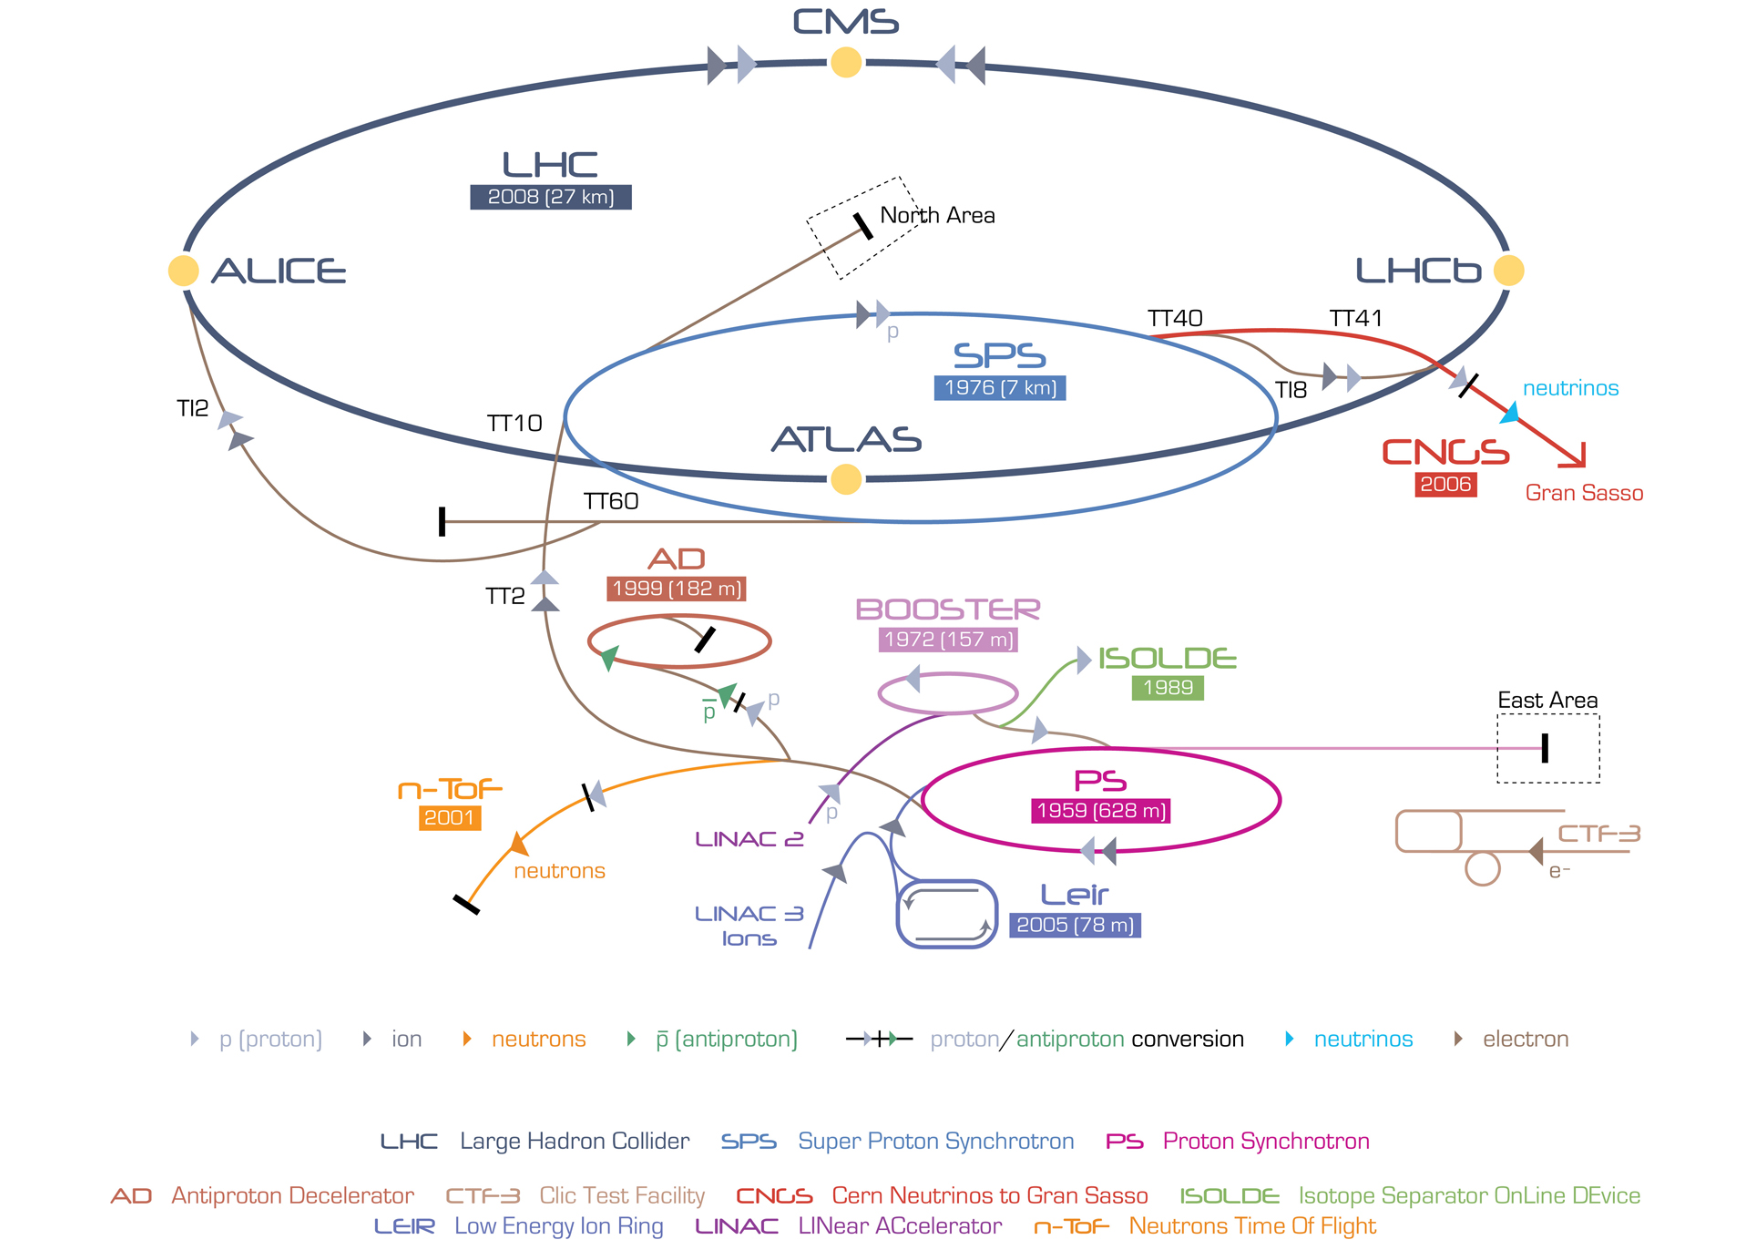
\includegraphics[width=12.cm]{./Version1/FigChapter4/FigureLHC}
\caption{ The CERN accelerator complex \cite{cite:LHCfig}}
\label{fig:lhc}
\end{center}
\end{figure}

The CERN accelerator complex is shown in the Figure \ref{fig:lhc}. The sequence of injection of bunches into the LHC is started from acceleration in the LINAC (LINear ACcelerator )2, PS (Proton Synchrotron) booster, PS, and SPS (Super Proton Synchrotron) accelerators. The way to inject of heavy-ion bunches are different. The bunches pass the LINAC3 instead of LINAC2, LEIR (Low Energy Ion Ring), PS and SPS accelerators \cite{cite:LHCinfo}. 


The first pp collisions at 900 GeV center of mass energy were delivered by the LHC on September 10th 2008. Nine days later, the operations were interrupted due to a failure in an electrical connection between two magnets. The machine operators spent over a year repairing and consolidating the accelerator. On November, 2009 low energy proton beams circulated again, and a few days later, by achieving the energy of 1.18 TeV per proton beam, LHC became the most powerful accelerator in the world. The first pp collisions at center of mass energy of 7 TeV were delivered in March 2010, and the first Pb--Pb collisions at center of mass energy of 2.76 TeV per nucleon pair in November 2010. 

In 2010 the integrated luminosity delivered by the LHC was $\sim$ 48 $pb^{-1}$ for pp collisions at \s = 7 TeV ($\sim$ 0.5 $pb^{-1}$ in ALICE) and $\sim$ 10 $\mu b^{-1}$ for Pb--Pb at \snn = 2.76 TeV ($\sim$ 9 $\mu b^{-1}$ in ALICE) \cite{cite:ALICEPerformance}. In 2011 the beam energy was the same as in 2010 both for pp and Pb--Pb. The performance of the LHC improved in terms of luminosity with $\sim$ 5.61 $fb^{-1}$ for pp ($\sim$ 4.9 $pb^{-1}$ in ALICE) and $\sim$ 166 $\mu b^{-1}$ for Pb--Pb collisions ($\sim$ 146 $\mu b^{-1}$ in ALICE). In 2012, the centre-of-mass energy for pp collisions was brought to 8 TeV and the integrated luminosity (up to December 2012, end of the pp program) was $\sim$ 23.3 $fb^{-1}$ ($\sim$ 10 $pb^{-1}$ in ALICE). A pilot p--Pb run operated at \snn = 5.02 TeV on September 2012, followed by a long p--Pb run on February 2013 with a delivered luminosity of 14 $nb^{-1}$. A very short pp run at \s = 2.76 TeV ended the Run1 of the LHC program, marking the start of the first long shutdown (LS1) until the end of 2014. %Despite its excellent performance, the LHC has not yet achieved the nominal parameters (\s, $L$), that is the main goal for the next ignition of the machine in 2015. 

The LHC produces collisions in four so called Interaction Points (IPs) in correspondence of which are located six detectors of different dimensions and with different goals, all able to study the products of the interactions. These are: \\

\textbf{ALICE (A Large Ion Collider Experiment-IP$_{2}$)} \cite{cite:proposalALICE} is devoted heavy-ion experiment intended to investicate strongly interacting matter at very high energy density. It explores the phase transition to the QGP phase diagram and its properties. Furthermore, the ALICE study the results of pp and p--Pb collisions, as a reference for heavy-ion measurements. ALICE is able to measure identified particles by using excellent particle identification capability and its acceptance reached to very low transverse momenta. \\

\textbf{ATLAS (A Toroidal LHC ApparatuS-IP$_{1}$)} and \textbf{CMS (Compact Muon Solenoid - IP$_{5}$) }\cite{cite:proposalATLAS}\cite{cite:proposalCMS} are built to cover the widest possible range of physics at the LHC and they are dedicated to collect results from pp collisions.  Specific topics are the beyond the Standard Model and serch for the Higgs boson. \\

\textbf{LHCb (The Large Hadron Collider beauty experiment-IP$_{8}$)} \cite{cite:proposalLHCb} is a dedicated experiment for the study of heavy flavor physics at the LHC. In particular, the experiment focuses on the study of CP violation and rare decays of beauty and charm particles, to test the Standard Model and to search for evidence of New Physics. The LHCb physics program is complementary to the flavor physics studies and to the direct exploration for new particles performed at ATLAS and CMS. \\

%\textbf{LHCf (Large Hadron Collider forward experiment-IP$_{1}$)} \cite{cite:proposalLHCf} measures forward particles created during LHC collisions to provide further understanding of high energy cosmic rays. The detector is placed close to the ATLAS experiment. \\

\textbf{TOTEM (TOTal Elastic and diffractive cross-section Measurement-IP$_{5}$)} \cite{cite:proposalTOTEM} is dedicated to the measurement of the total pp cross-section, study of elastic and diffractive scattering. The detector is built at the same interaction point of the CMS experiment. \\

\subsection{The ALICE project}
The main gold of the ALICE experiment at the LHC \cite{cite:ALICE} is study of matter produced extreme conditions of temperature and energy density from ultra-relativistic heavy-ion collisions. The purpose is to inspect the existence of a phase transition from the hadronic matter to the QGP which was proposed by QCD prediction. Because only ALICE is the LHC experiment specifically designed for Pb--Pb collisions, it has to be able to cope with the large multiplicities associated with these collision systems and at the same time has to cover as many QGP-related observables as possible. ALICE is also interested in the results of pp interactions, since these are the baseline for the results obtained Pb--Pb collisions. It is not only crucial for comparison with Pb--Pb but also can be used to tune Monte Carlo models. 

In comparison with the other experiments, ALICE is able to provide an excellent Particle IDentification (PID) performance obtained by combination of different PID techniques from various detectors that are optimized in different momentum ($\ensuremath{p}$) regions.

\subsubsection{ALICE detector}\label{label:alice}
ALICE is a complex of 14 detector subsystems (Figure \ref{fig:alicedetector}) that can be categorized in three groups: \\

\textbf{Central detectors} are installed in a solenoid magnet which gives 0.5 T magnetic field and covered pseudo-rapidity interval is -0.9 $< \eta <$0.9 (corresponding to a polar acceptance $\pi$/4 $< \theta <$ 3$\pi$/4). The acceptance in azimuthal angle is 2$\pi$. The central detectors are mainly used to vertex reconstruction, tracking, particle identification and momentum measurement. From interaction region to outward region of detector, there are several detectors explained below:



\begin{itemize}
\item Inner Tracking System (ITS)
\item Time Projection Chamber (TPC)
\item Transition Radiation Detector (TRD)
\item Time Of Flight (TOF)
\end{itemize}

Following three detectors have limited azimuthal acceptance in the  mid-rapidity region:

\begin{itemize}
\item High Momentum Particle Identification Detector (HMPID)
\item PHOton Spectrometer (POHS)
\item ElectroMagnetic CALorimeter (EMCAL)
\end{itemize}


\textbf{Muon spectrometer} is located in the forward pseudo-rapidity region (-4.0 $< \eta <$ -2.5) and is made up of a dipole magnet and tracking and trigger chambers. It has been optimized and configured to extract single muons and to reconstruct heavy quark resonances (such as J/$\Psi$ through their $\mu^{+}\mu^{-}$ decay channel). \\

\textbf{Forward detectors} are placed in the high pseudo-rapidity area (small angles with respect to the beam pipe). They are used to measure global event characteristics and for triggering.

\begin{itemize}
\item Time Zero (T0) measures the time of events with precision of the order of tens of picoseconds, as needed by TOF.
\item VZERO (V0) rejects the backgrounds coming from beam-Gas interaction and trigger minimum bias events.
\item Forward Multiplicity Detector (FMD) gives multiplicity information and it covers large fraction of the solid angle (-3.4 $< \eta <$ -1.7 and 1.7 $< \eta <$ 5).
\item Photon Multiplicity Detector (PMD) measures the spatial distribution of photons on an event-by-event basis in 2.3 $< \eta <$ 3.7 region.
\item Zero Degree Calorimeter (ZDC) is used to measure and trigger on the impact parameter. The ZDC consists of two calorimeters, one for neutrons (ZDC:ZN) and another one for protons (ZDC:ZP), and includes also an electromagnetic calorimeter (ZEM)
\end{itemize}

\begin{figure}[htbp]
\begin{center}
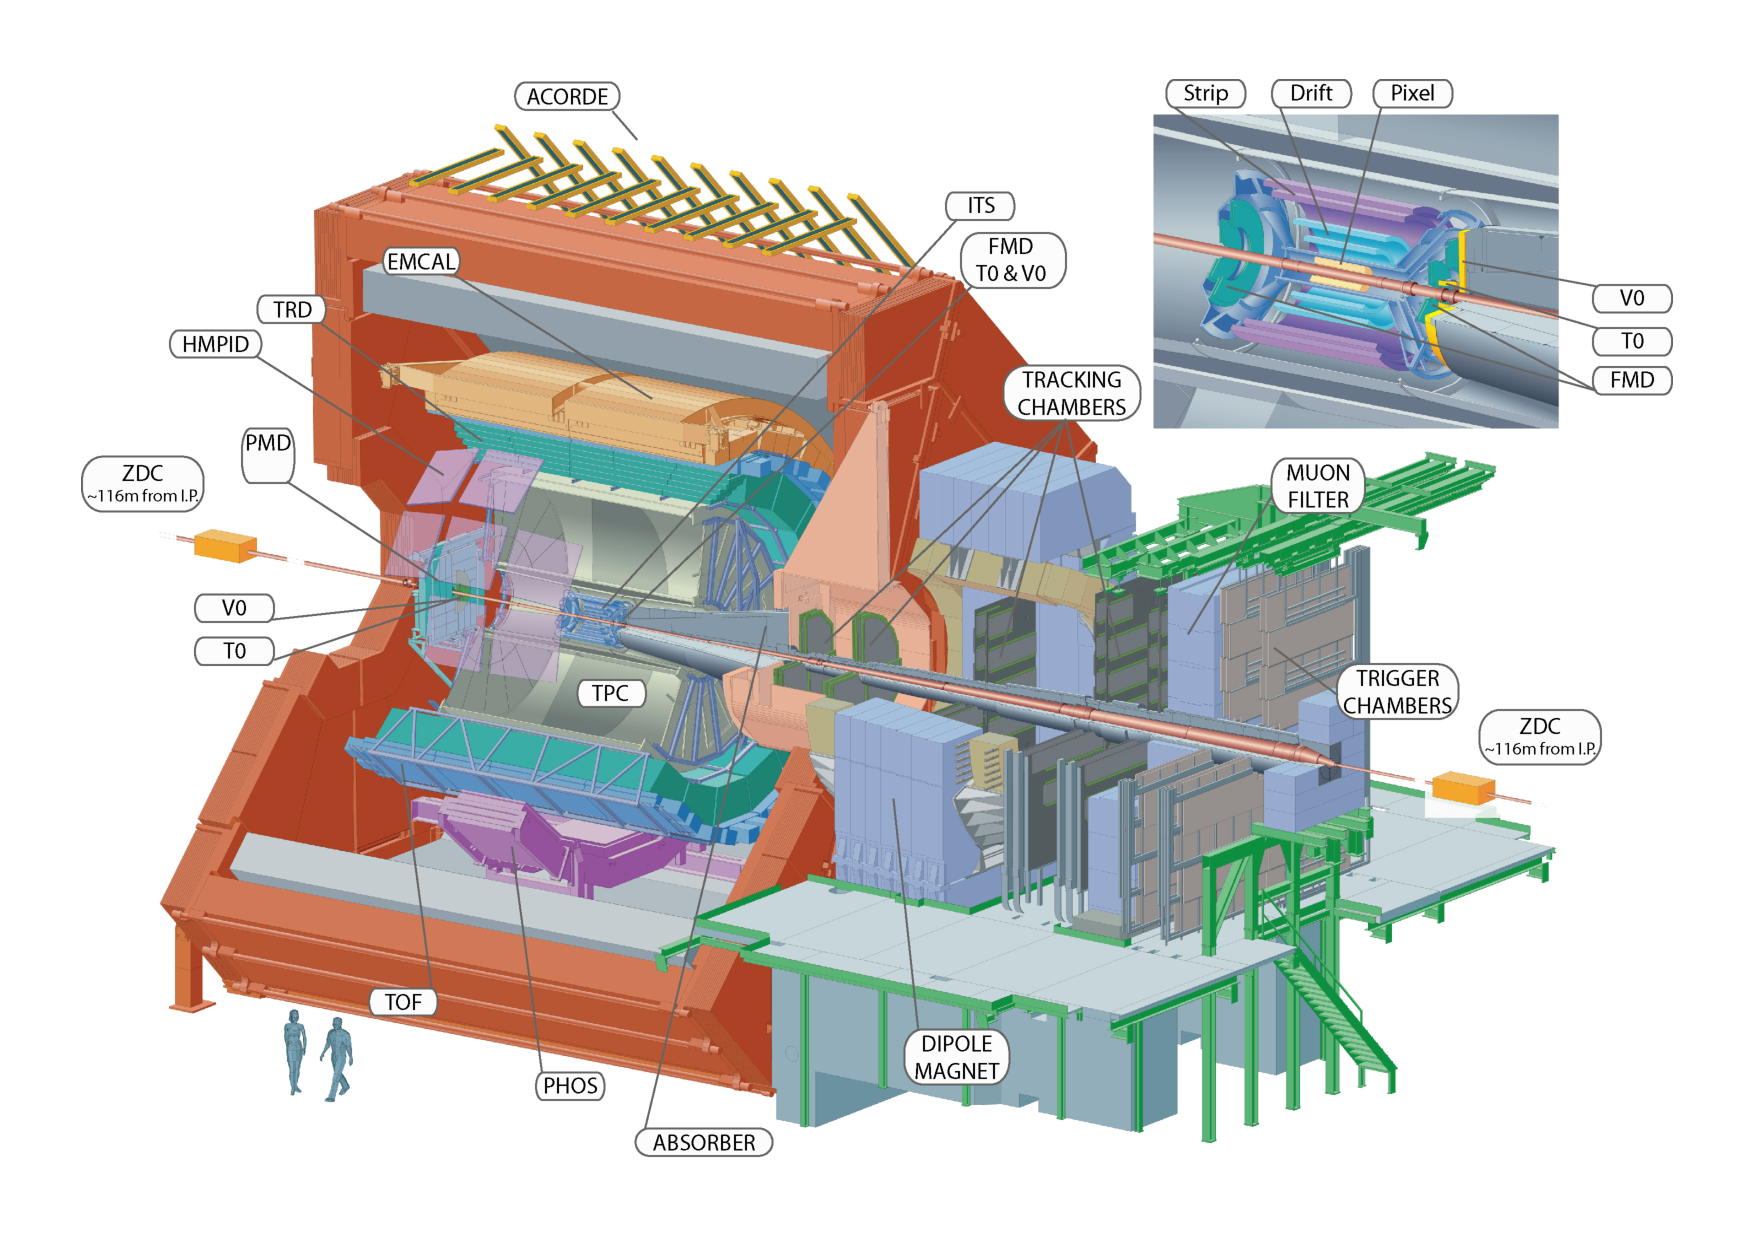
\includegraphics[width=14.cm]{./Version1/FigChapter4/FigureALICE}
\caption{ The ALICE detector}
\label{fig:alicedetector}
\end{center}
\end{figure}


The ALICE global coordinate system \cite{cite:ALICEcoord} is a right-handed orthogonal Cartesian system with the origin X, Y, Z = 0 at the centre of the detector. The three Cartesian axes are defined as follows: the X axis pointing towards the center of the LHC, the Y axis pointing upward and the Z axis parallel to the local mean beam line pointing in the direction opposite to the muon spectrometer. The azi- muthal angle increases counter-clockwise from the positive X axis ( $\Phi$= 0) to the positive Y axis (  $\Phi$ = $\pi$/2) with the observer standing at positive Z and looking at negative Z; the polar angle increases from the positive Z axis ($\theta$ = 0) to the X-Y plane ($\theta$ = $\pi$/2) and to the negative Z axis ($\theta$ = $\pi$).

In the following Sections more specific descriptions of the detectors used in the identification of the \xis baryons and in the determination of the characteristics of typical collisions will be given. \\

{\Large\textsl{ITS}}\\
The ITS \cite{cite:ALICE} (Figure \ref{fig:its}) is the barrel detector which is closest to the beam pipe. Its main purposes are:

\begin{itemize}
\item to contribute to the global tracking with the TPC by improving the angle and momentum resolution
\item to reconstruct the position of the primary interaction vertex
\item to reconstruct strange particle decays and secondary vertices from decays of heavy-flavor
\item to track and identify particles with momentum below 100 \mmass
\item to improve the momentum, impact parameter and angle resolution for the measurement of high \pt particles performed with the TPC
\item to reconstruct particles traversing dead regions of the TPC
\end{itemize}


\begin{figure}[htbp]
\begin{center}
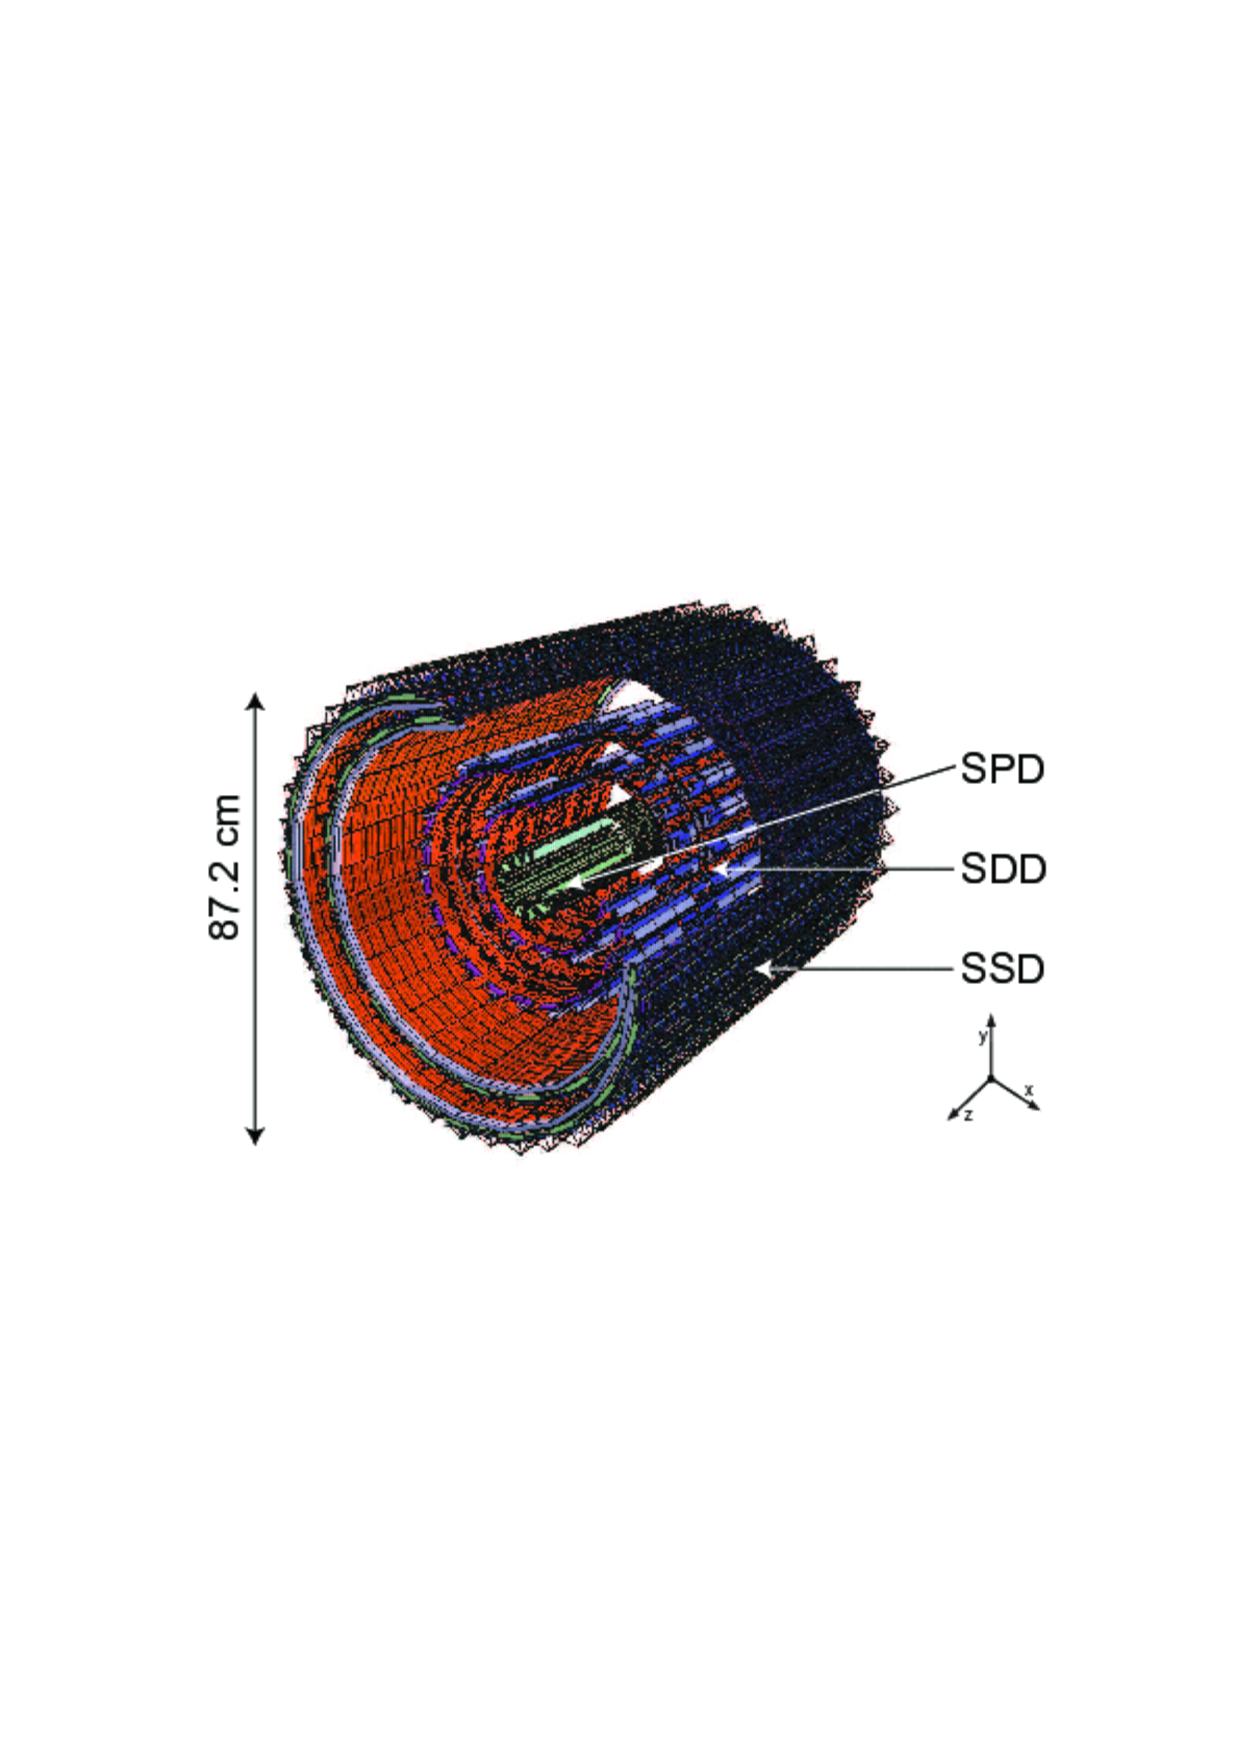
\includegraphics[width=12.cm]{./Version1/FigChapter4/FigureITS}
\caption{Schematic view of the ITS \cite{cite:ITS}}
\label{fig:its}
\end{center}
\end{figure}


The ITS encircles the beam pipe which is a 800 $\mu$m thickness cylinder shape with an outer diameter of 2.9 cm. It consists of six layers of silicon detectors placed at radii from $\sim$4 cm to $\sim$43 cm. The two innermost layers are Silicon Pixel Detectors (SPD), Silicon Drift Detectors (SDD) is placed in middle and the two outmost layers are Silicon micro-Strip Detectors (SSD). 

\begin{figure}[htbp]
\begin{center}
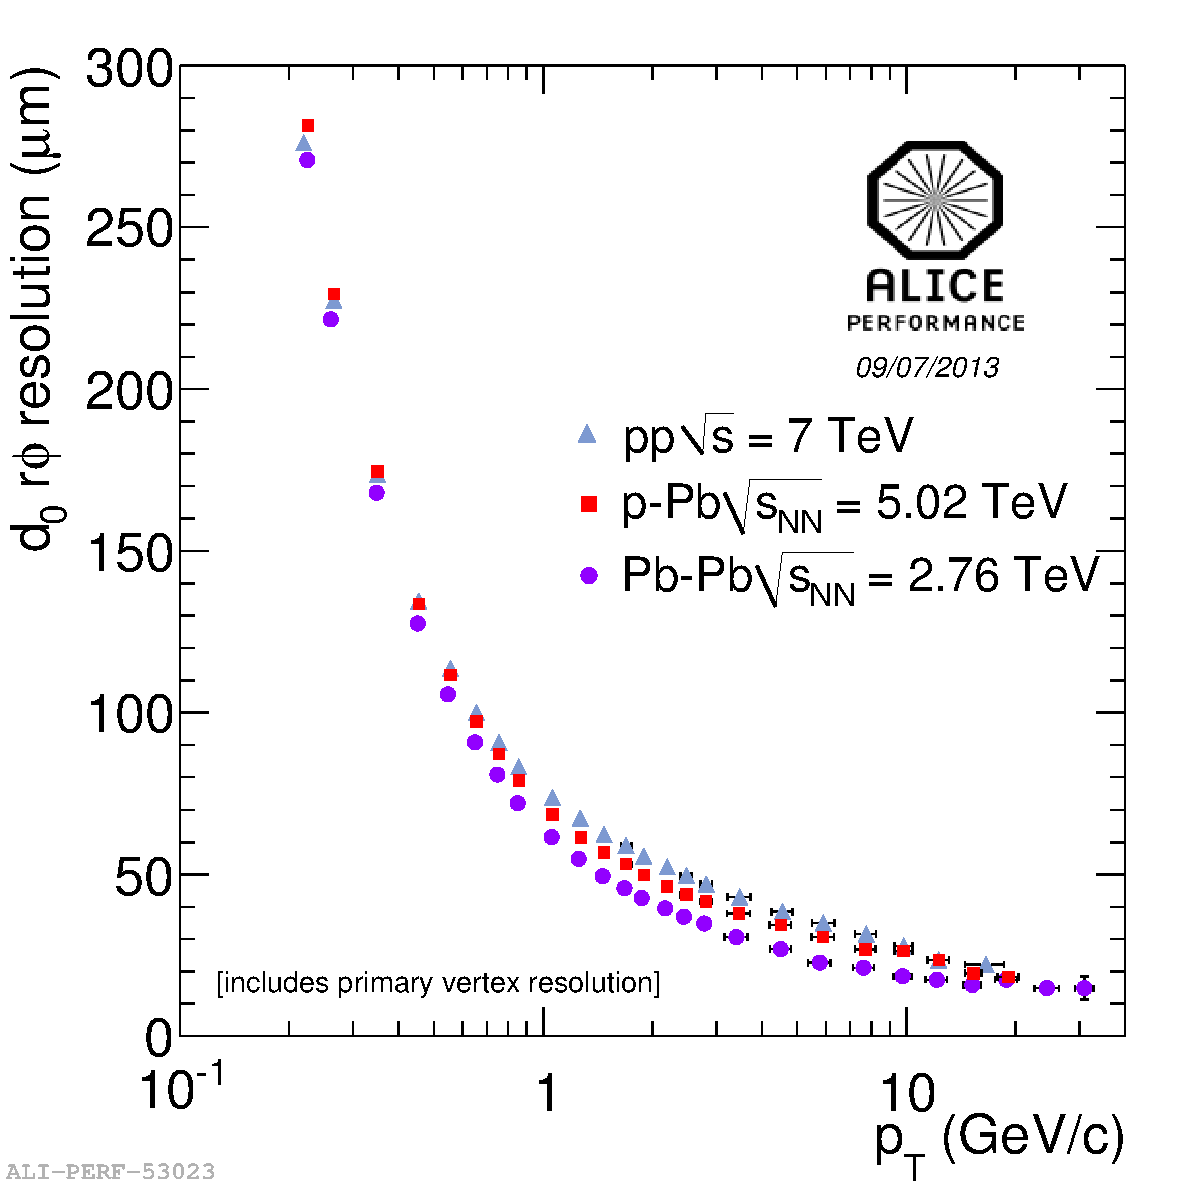
\includegraphics[width=10.cm]{./Version1/FigChapter4/ITSPerformance}
\caption{Track impact parameter resolution (r$\phi$) in the transverse plane as function of  \pt~for charged particle}
\label{fig:itsperformance}
\end{center}
\end{figure}


The amount of material in the detector has to be minimized because the momentum and impact parameter resolutions for low momentum particles are dominated by multiple scattering effects. The track impact parameter resolution as function of \pt~ is shown in Figure \ref{fig:itsperformance}. The ITS detector has a spatial resolution better than 70 $\mu$m in the (r$\phi$) for \pt $>$ 1 GeV/$c$. \\





{\Large\textsl{TPC}}\\

The TPC \cite{cite:TPC} (Figure \ref{fig:tpc}) is the main tracking detector of the central barrel optimized to measure charged particle momentum with good track separation, particle identification and vertex determination. In order to get the track in high multiplicity environment of Pb--Pb collisions, the TPC was designed to have an excellent tracking performance. For such reason, it was constructed as a drift chamber in 5 m cylindrical shape. The inner radius is r$_{in}$ $\sim$ 85 cm decided by the maximum acceptable track density and the most outer radius is r$_{out}$ $\sim$ 250 cm to minimize track length for which d$E$/d$x$ is $<$ 10\%. The volume of TPC is 90 m$^{3}$ and it is filled by Ne/CO$_{2}$/N$_{2}$. The readout chambers are installed at the two endplates of the cylinder. Their design is based on the Multi-Wire Proportional Chamber (MWPC) technique with pad readout. The TPC has good d$E$/d$x$ resolution as results it is able to identify particles with \pt $<$ 1 GeV/$c$ on a track-by-track basis.

\begin{figure}[htbp]
\begin{center}
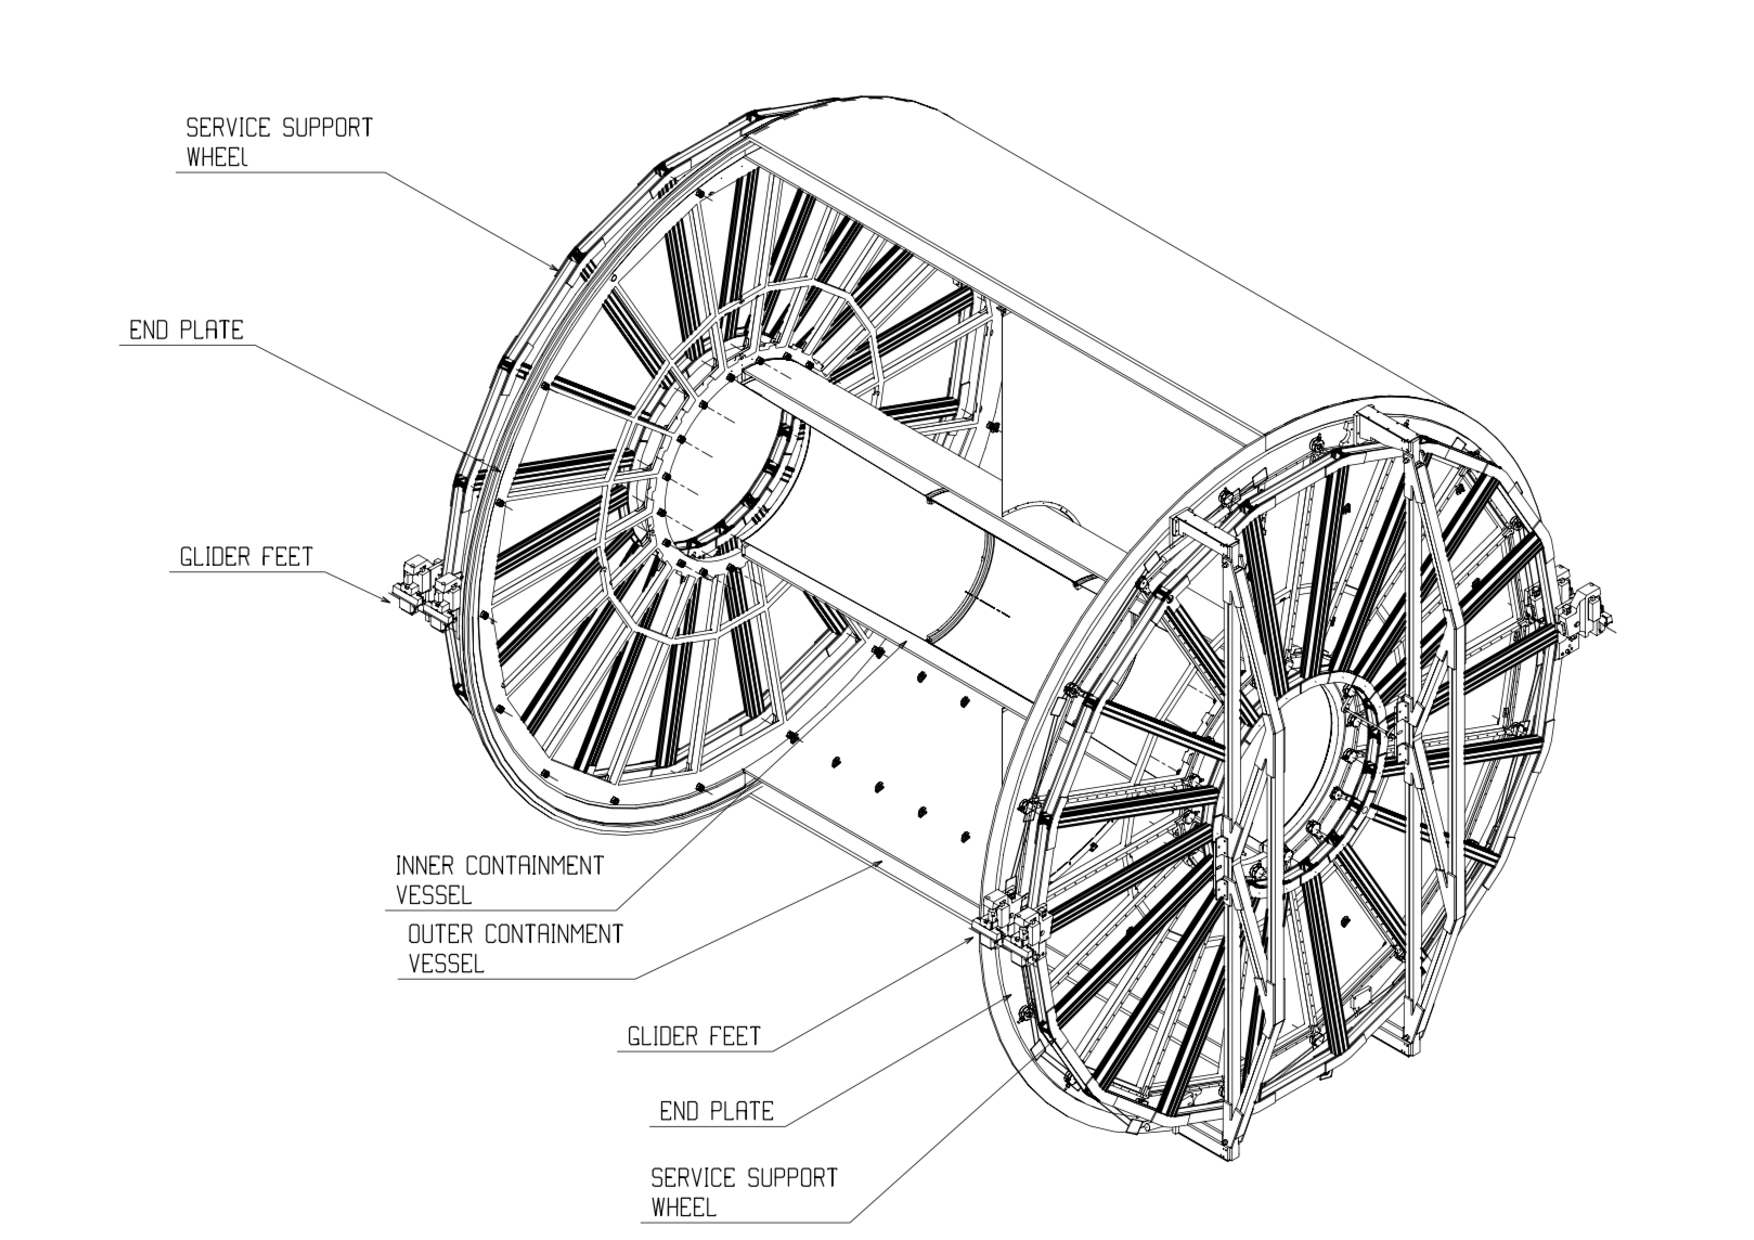
\includegraphics[width=10.cm]{./Version1/FigChapter4/FigureTPC}
\caption{Schematic view of the TPC}
\label{fig:tpc}
\end{center}
\end{figure}


The gas in the detector is ionized by charged particle traveling through the TPC. The measurement of this loss of energy is what we need to identify a particle. The physics observable in this case is the energy loss per unit length, within the matter crossed by the charged particle, which we call specific energy loss, also denoted by dE/dx. This is described by the Beth--Bloch equation, \ref{eq:BB}, that highlights the key of the identification technique: this observable depends only on the charge and on velocity ($\beta$) of the particle, which, in turn, depends only on the momentum and the mass of the ionizing particle. Since momentum is already known due to track curvature and charge is unitary for most measured tracks, measuring the dE/dx allows us to indirectly determine mass and thus determine the particle species.
The Bethe-Bloch equation gives the mean specific energy loss:
\begin{equation}\label{eq:BB}
- \langle\frac{dE}{dx}\rangle = k_{1} \cdot z^{2} \frac{Z}{A} \cdot \frac{1}{\beta^{2}}[\frac{1}{2}ln(k_{2}\cdot m_{e}c^{2}\cdot \beta^{2} \gamma^{2})-\beta^{2}+k_{3}]
\end{equation}

where $\beta\gamma$ = $\ensuremath{p}$/Mc and:
Z: atomic number of the ionized gas (in this case Ne/CO$_{2}$/N$_{2}$)\\
A: mass number of the ionized gas (g/mol)\\
m$_{e}$: electron mass\\
z: electric charge of the ionizing particle in unit of electron charge e\\
M: ionizing particle mass\\
$\ensuremath{p}$: ionizing particle momentum\\
$\beta$: ionizing particle velocity normalized to the light velocity c\\
$\gamma$ = 1/$\sqrt{1-\beta^{2}}$, Lorent factor\\
k$_{1}$, k$_{2}$, k$_{3}$: constants depending on the ionized medium\\ 


For a given ionizing particle mass hypothesis, a given momentum and a given length of the trajectory in the ionizing medium, the total charge deposited along the trajectory is subject to statistical fluctuations. This random variable follows a Landau distribution, that give us the opportunity to measure the mean value hdE/dxi. The long tail of the Landau distribution is usually truncated at 50\%-70\% of the collected signal. 

\begin{figure}[htbp]
\begin{center}
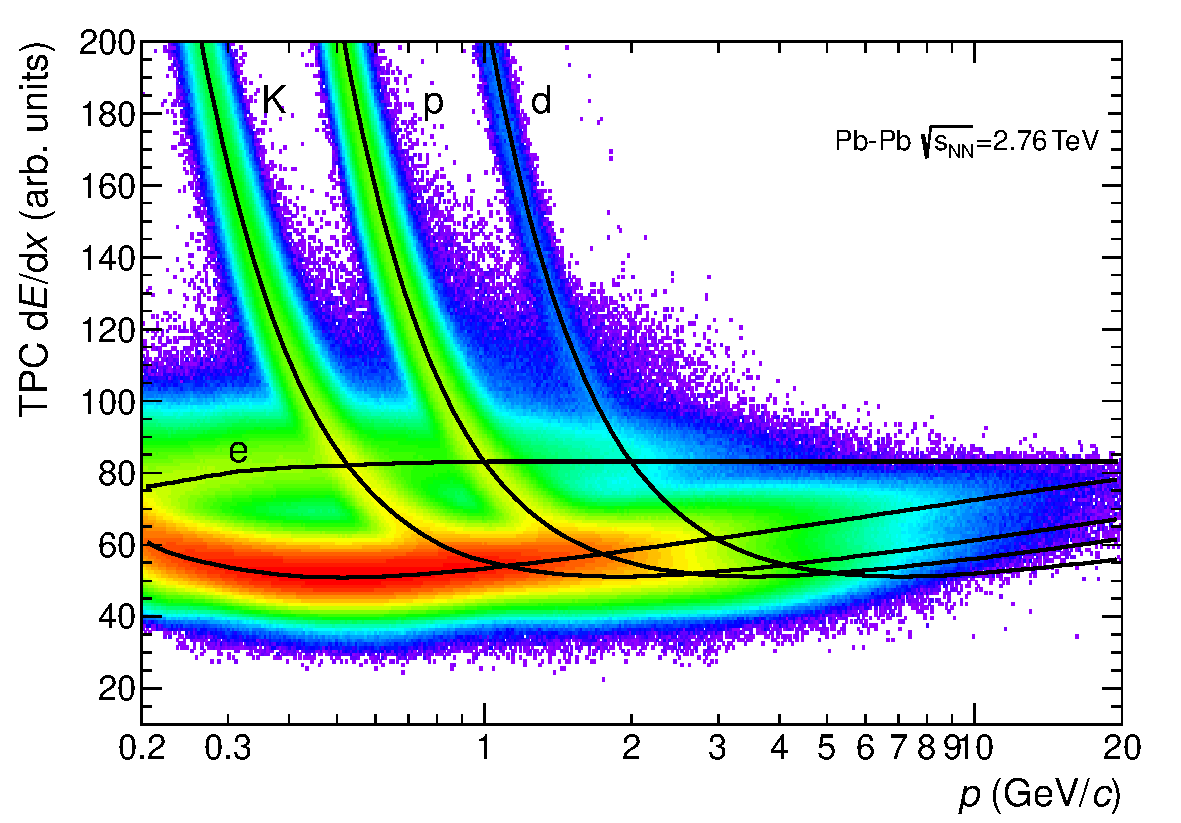
\includegraphics[width=10.cm]{./Version1/FigChapter4/TPCPID}
\caption{Specific energy loss (d$E$/d$x$) in the TPC as a function of momentum in Pb--Pb collisions at \snn= 2.76 TeV. The lines show the parameterizations of the expected mean energy loss.}
\label{fig:tpcpidPbPb}
\end{center}
\end{figure}

The specific energy loss in the TPC as a function of momentum is shown in Figure \ref{fig:tpcpidPbPb}. The different bands characteristic for e$^{\pm}$, $\pi^{\pm}$, K$^{\pm}$, p$^{\pm}$ are clearly visible. These are the evidence of the statistical distribution of the measured energy loss around the expected mean value. The expected value correspond to the prediction by a Bethe--Bloch experimental parametrization (superimposed as black lines in the Figure). For a track within the TPC the relevant quantity to be considered for PID is the difference between the specific energy loss measured by detector and the corresponding predicted value, by the Bethe-Bloch parametrization for a given measured momentum. If normalized to the resolution of the d$E$/d$x$ measurement in the TPC, this difference could be expressed in number of $\sigma$(see Equation \ref{eq:nsigma}). In this way it is possible to estimate more quantitatively the goodness of a mass hypothesis. This also gives us the possibility to choose the strictness we want to adopt in the identification of a particle (n$_{\sigma}$ , n = 2, 3, 4):

\begin{equation}\label{eq:nsigma}
n_{\sigma} = \frac{(dE/dx)_{measured}-(dE/dx)_{Bethe-Bloch}}{\sigma_{TPC}}
\end{equation}


{\Large\textsl{V0}}\\
The VZERO detector \cite{cite:V0} consists of two segmented arrays of plastic scintillator counters, called VZERO-A and VZERO-C, placed near the beam-pipe on each side of the interaction point: one at Z = 340 cm, covering the pseudo-rapidity range (2.8 $< \eta <$ 5.1), and the other at Z = -90 cm in front of the absorber, covering the pseudo-rapidity range (-3.7 $< \eta <$ -1.7). 

%Each of VZERO (A or C) consists of 32 channels distributed in 4 rings with separation of 45$^{\circ}$. The Wave-Length Shifting (WLS) fibers are embedded in both face of the detector. Clear fibers collect and transport the signal to photomultipliers 3 - 5 m far from the detector, inside the L3 magnet. The counters have a time resolution better than 1 ns. Their response is recorded in a time window of 25 ns around the nominal beam crossing time.

By measuring the relative time of flight, the VZERO reject background from beam-gas collisions. (see, Figure \ref{fig:v0}) The time of flight of particles coming from the interaction point to the VZERO-A is $\sim$ 11 ns while VZERP-C is 3 ns. If the beam-gas collision takes place outside the region between the two arrays, particles arrive 6 ns before or after the time of a beam-beam collisions. When the beam-gas collision takes place outside the region between the two arrays, particles arrive 6 ns before or after the time of a beam-beam collision as shown in Figure \ref{fig:v0time.}

\begin{figure}[htbp]
\begin{center}
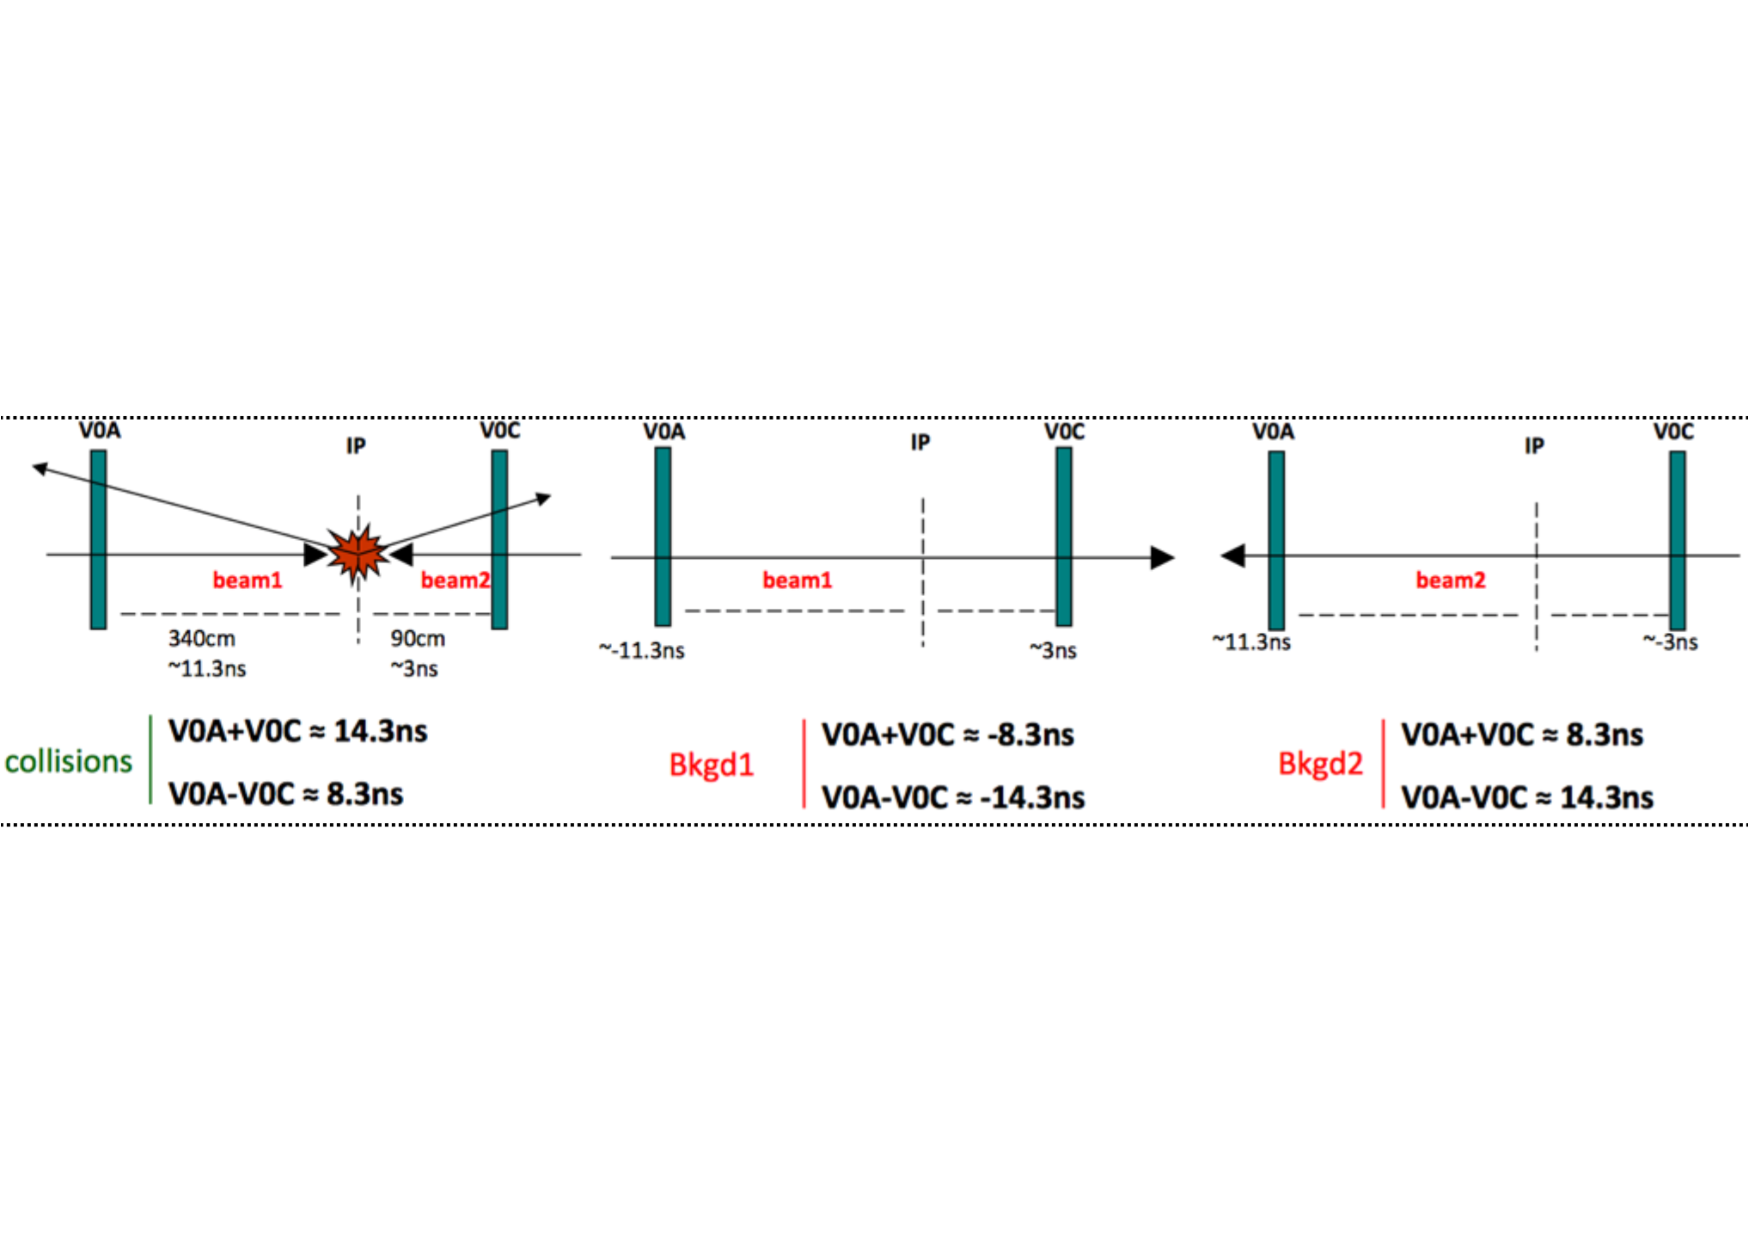
\includegraphics[width=14.cm]{./Version1/FigChapter4/V0time}
\caption{Sketch of events collisions at (8.3 ns, 14.3 ns) is shown in left, background from Beam 1 at (-14.3 ns, -8.3 ns) in in middel and background from Beam 2 at (14.3 ns, 8.3 ns) is in right.}
\label{fig:v0time}
\end{center}
\end{figure}

\begin{figure}[htbp]
\begin{center}
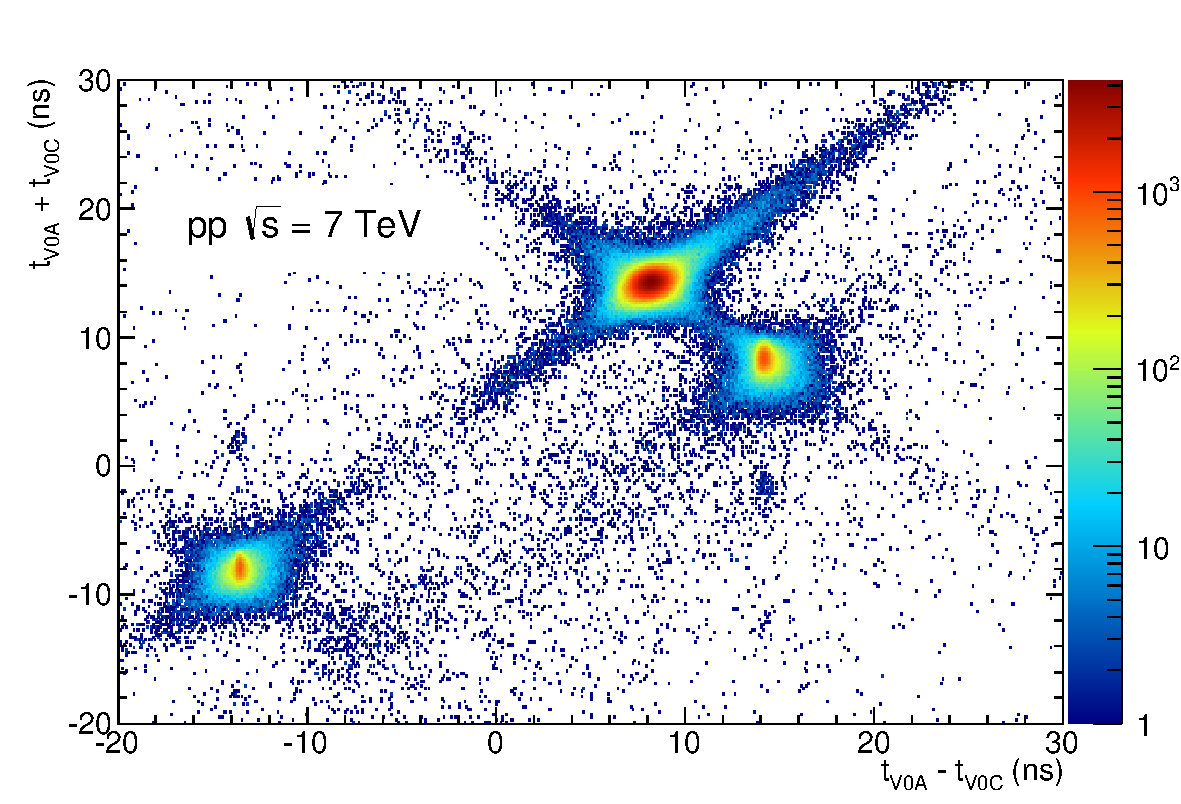
\includegraphics[width=10.cm]{./Version1/FigChapter4/FigureV0}
\caption{Correlation between the sum (y-axis) and difference (x-axis) of signal times in V0A and V0C. The signals in center come from beam-beam interactions, the signal in left is background from Beam1 and background from Beam2 is shown in right hand.}
\label{fig:v0}
\end{center}
\end{figure}



As the VZERO is a trigger detector, it will provide a minimum-bias trigger for all colliding systems to the central barrel detectors and different centrality triggers in p--Pb and Pb--Pb collisions (e.g. multiplicity, central and semi-central).  

The first parameter to be determined in A--A(p--A) collisions is the centrality(multipliciy). This is defined according to the value of the impact parameter, b, and provides a geometrical scale of the overlapping region between the colliding nuclei: a collision will be defined from central to peripheral, as the impact parameter increases. The centrality of a collision is not directly available and must be deduced from a combination of experimentally measured quantities and Monte Carlo simulations.

%There are a number of observables that can be measured and used as centrality estimators. The charged-particle multiplicity N$_{ch}$ and the transverse energy E$_{\mathrm{T}}$ measured around mid-rapidity are measurable quantities related to the energy deposited in the interaction region (these are therefore related to N$_{part}$). 

The charged-particle multiplicity N$_{ch}$ is observable that can be measured and used as centrality estimator and it is related to  N$_{part}$. The variables increase significantly increasing the centrality of the collisions. Another measurable quantity to estimate the centrality is the zero-degree energy EZDC, namely the energy carried by spectator nucleons N$_{spec}$ = 2A - N$_{part}$ = E$_{ZDC}$/E$_{A}$, where E$_{A}$ is the beam energy per nucleon.
Typically a measured distribution of one of the previous observables is mapped to the corresponding distribution obtained from phenomenological Glauber calculations. The Glauber model \cite{cite:glauber,cite:glauber1} uses a semi-classical approach: the A--A collision is assumed to be an incoherent superposition of N elementary nucleon- nucleon collisions. The main parameters of the model are the inelastic nucleon-nucleon collision cross-section $\sigma_{n}$ and the nuclear density distribution $\rho$(r). In practice, the simulated distribution well reproduce the measured distribution or the latter is fitted with an analytical function. The experimental distribution can then be divided in classes with sharp cuts on the measured observable (E$_{ZDC}$, E$_{T}$ or N$_{ch}$). These "centrality" classes will correspond to well defined percentage of the integral of the distribution. A given centrality class in the measured distribution, corresponds to the same class in the simulated distribution, where the main geometrical variables (N$_{part}$, N$_{coll}$ and T$_{AA}$) can be determined. The number of classes that can be defined depends on the resolution achievable on the selection variable.
In the analysis described in this thesis the centrality(multiplicity) estimation is based on the measurement of the multiplicities from the VZERO scintillators \cite{cite:centralitypPb}\cite{cite:centralityPbPb}. This is the method that achieve the best centrality resolution: it ranges from 0.5\% in central to 2\% in peripheral collisions. Other methods, as the ones based on the E$_{ZDC}$ measurement or based on the estimate of the number of tracks in the SPD or TPC, are used to asses a systematic uncertainty on the centrality determination.
The distribution of the VZERO amplitudes is shown in Figure \ref{fig:centralityestimate} where the centrality(multiplicity) percentiles are also indicated. 

\begin{figure}[htbp]
\begin{center}
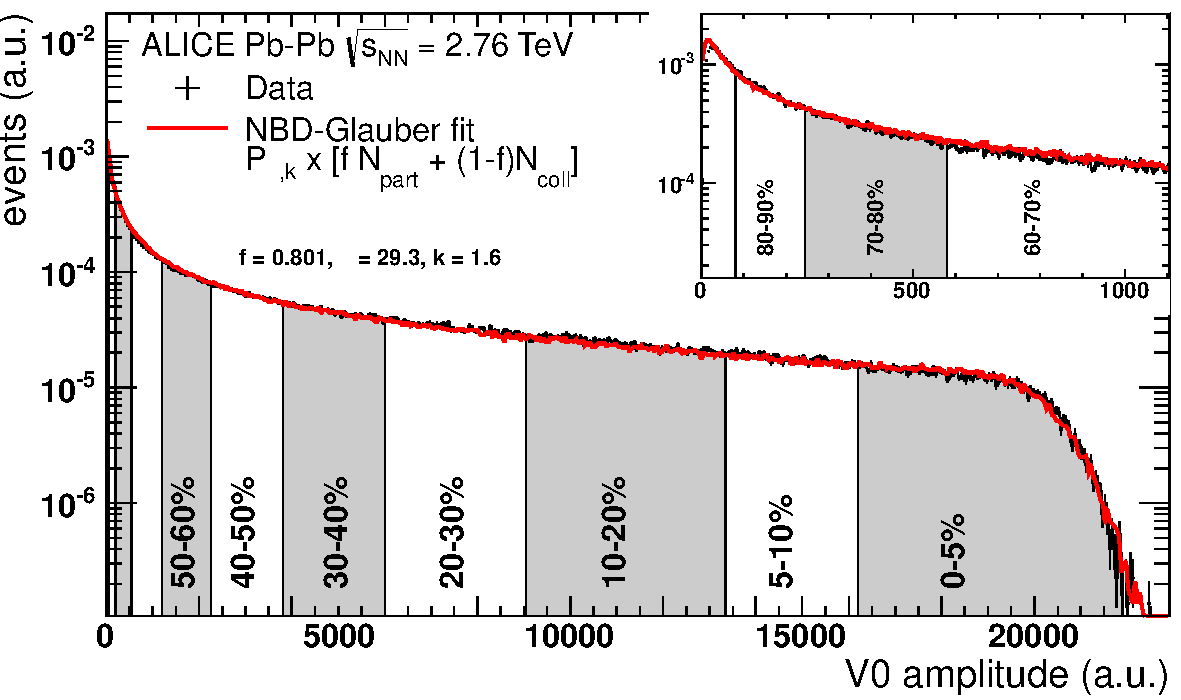
\includegraphics[width=12.cm]{./Version1/FigChapter4/CentralityPbPb}
\hspace{1.0cm}
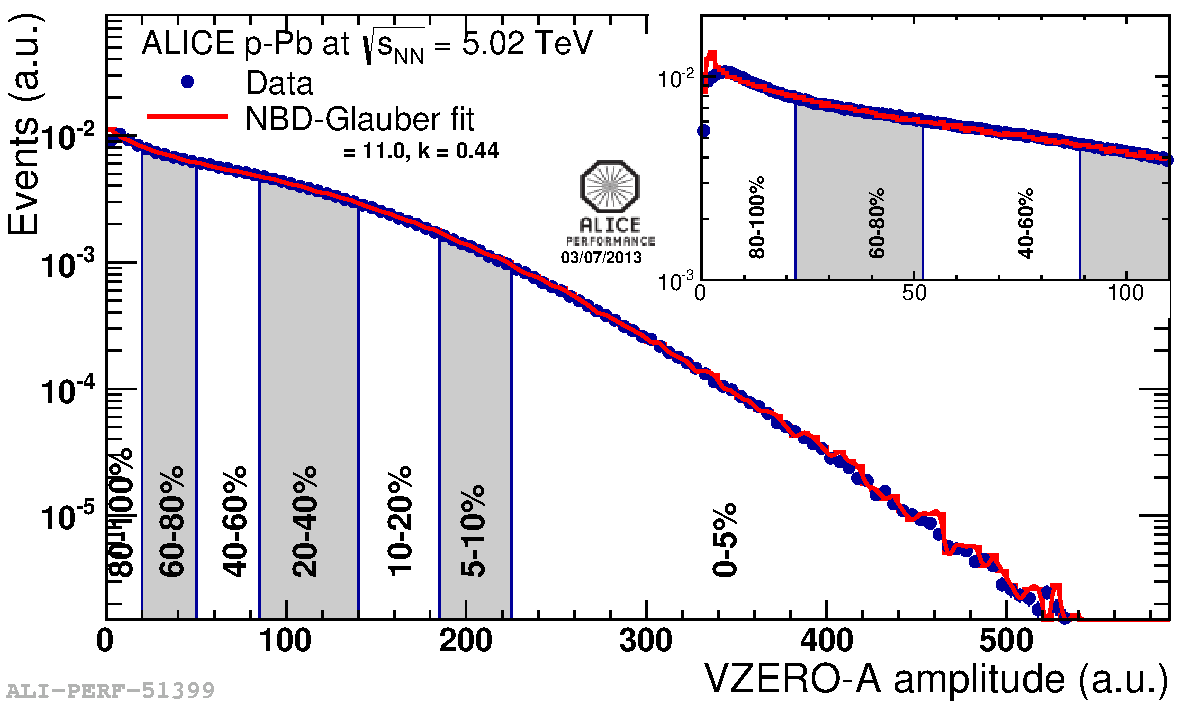
\includegraphics[width=12.cm]{./Version1/FigChapter4/CentralitypPb}
\caption{ Sume of V0A and V0C amplitude distribution in top and V0A amplitude distribution in bottom.}
\label{fig:centralityestimate}
\end{center}
\end{figure}

\newpage
\subsubsection{Data Acquisition (DAQ) and trigger system}\label{label:aliceDAQ}
The architecture of data acquisition is shown in Figure \ref{fig:daq}. The tasks of the ALICE DAQ system are the assembly of event informations from individual detectors into complete events (event building) as well as buffering and export of assembled events to permanent storage. 

The DAQ is geared to accumulate a data rate up to 1.25 GB/s in heavy-ion runs. The event is builded in several procedures. Data from each detectors is received by Detector Data Links (DDLs) on Local Data Concentrators (LDCs). And the LDCs collect the data into sub-events that are then shipped to Global Data Collectors (GDCs). A GDC receives all sub-events from a given event and assembles them into a complete event. These events are subsequently stored on a system called Transient Data Storage (TDS).


\begin{figure}[htbp]
\begin{center}
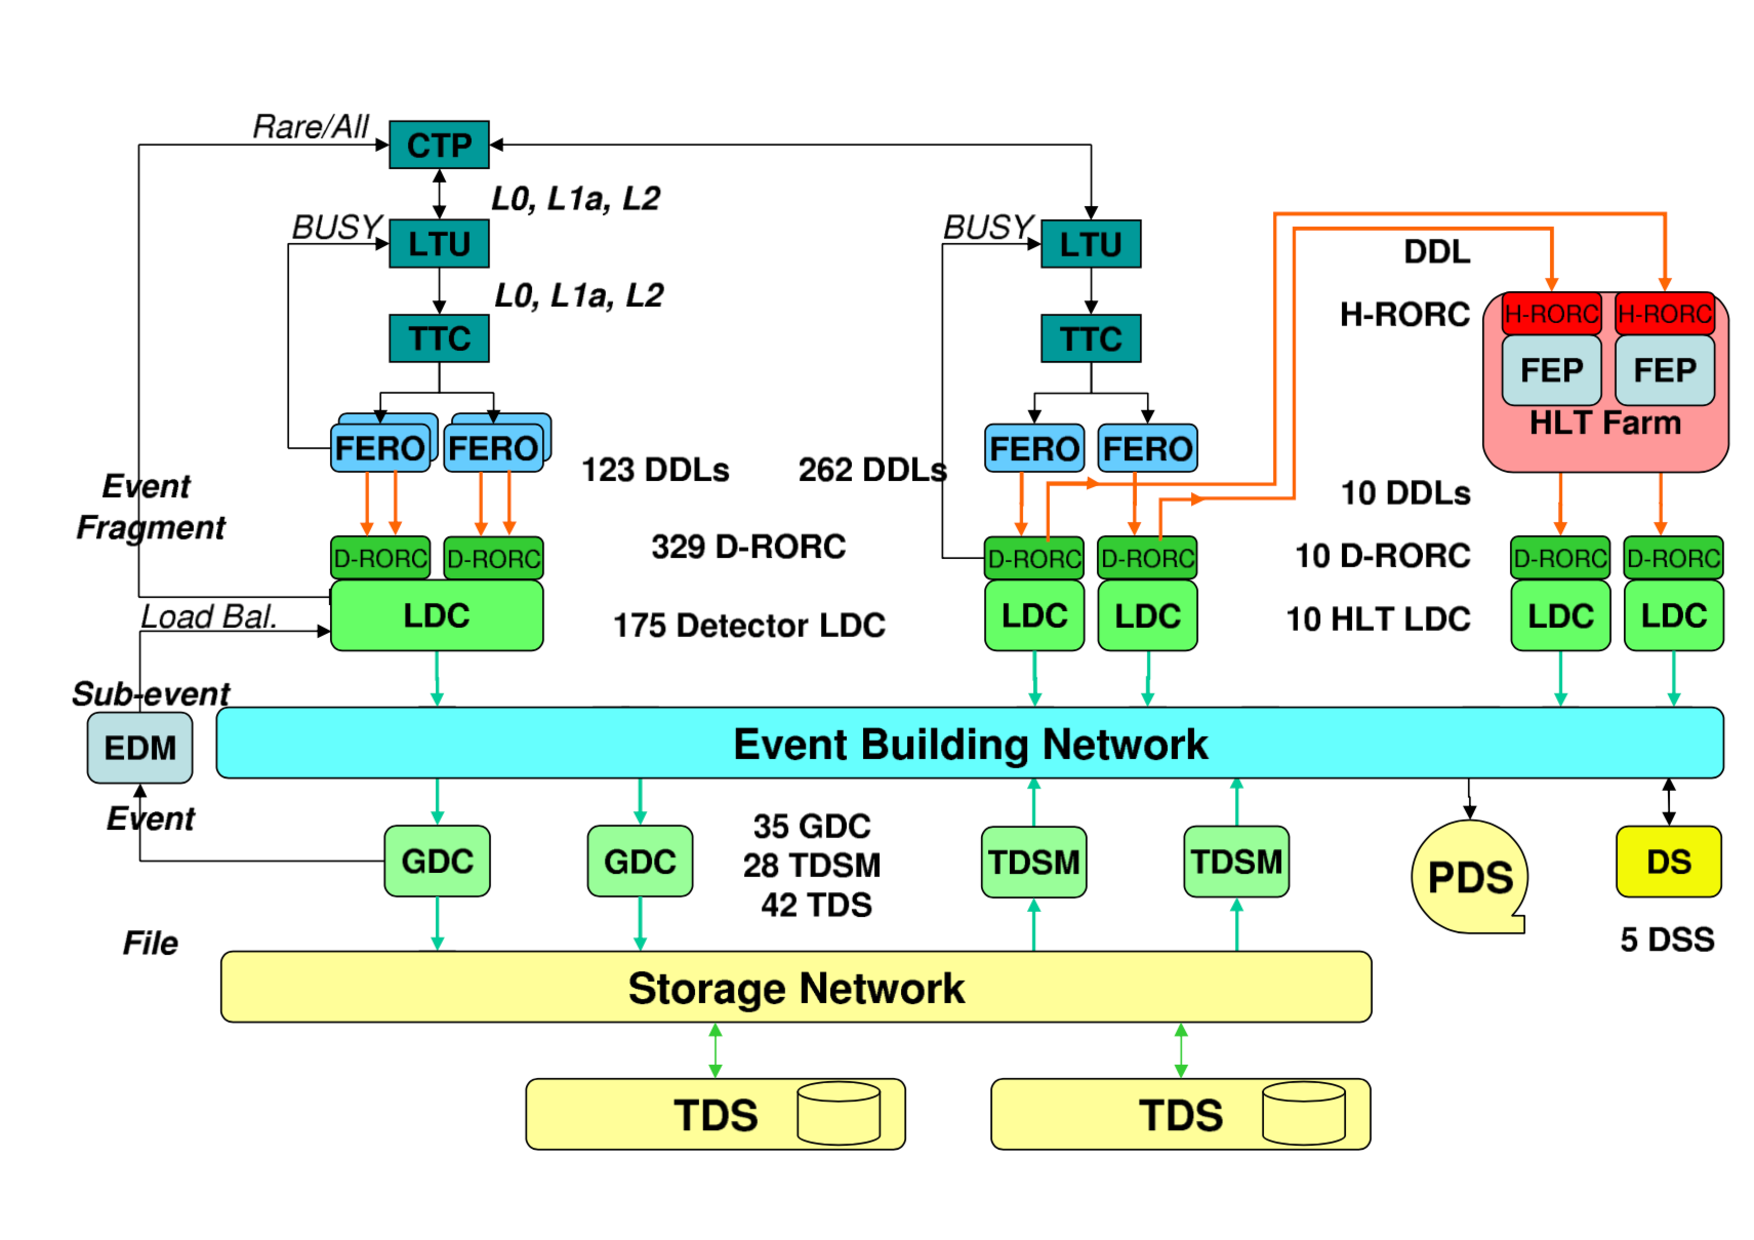
\includegraphics[width=14.cm]{./Version1/FigChapter4/FigureDAQ}
\caption{The overall architecture of the ALICE DAQ and the interface to the HLT system.}
\label{fig:daq}
\end{center}
\end{figure}

 ALICE can simultaneously take data in several partitions, where a set of detectors can store their outputs. Since a partition is a group of commonly controlled detectors, a given detector can only be active in one partition at a time. The active detectors in a given partition may be assigned to data taking groups called clusters, for which triggers can be defined. 
 
% Therefore, upon a trigger only a subset of the whole partition may be read out. Furthermore, a triggering detector does not have to be necessarily part of the partition.
ALICE has a two-layer trigger architecture \cite{cite:daq}. The low-level trigger is a hardware trigger called Central Trigger Processor (CTP). The High-Level Trigger (HLT) is implemented as a pure software trigger. The CTP combines inputs from different trigger sources, namely the various detectors. These inputs are single signals, like a hit in the detector, or, can be the result of fast calculation performed directly in the detectors. The HLT allows the implementation of sophisticated logic for the triggering. In contrast to the CTP which governs the readout of the detectors, the HLT receives a copy of the data read out from the detectors and processes them.

The hardware trigger combines the trigger signals of the various detectors to decide if an event is accepted, that means it is read out and written to disk. Several trigger levels reduce the event rate depending on the input signals. The first level, called L0, is delivered after 1.2 $\mu$s, while the second, called L1, after 6.5 $\mu$s. The final trigger, L2, is delivered after 100 $\mu$s, upon completion of the drift time in the TPC. Only after an L2 trigger the event is finally stored. The rates of different trigger classes are very different. By definition minimum-bias triggers have the highest rate, other triggers that look for rare signals are characterized by much lower rates. In order to cope with different scenarios, downscaling factors can be applied to the trigger classes individually, i.e. only every nth event fulfilling the trigger condition is read out. The total recording rate is limited by the maximum bandwidth of data that can be recorded to disk and tape.

The ALICE software trigger, called HLT, is a farm of multiprocessor computers. The aim is to have about 1000 PCs processing the data in parallel allowing an online analysis of the events. A trigger decision comes from the analysis of a more comprehensive set of information than what happens for the hardware trigger, giving the possibility to apply more sophisticated triggers. Examples include triggers on high energy jets or on muon pairs. Furthermore, the HLT can significantly reduce the event size by selecting regions of interest (partial readout of detectors) and by further compression of the data. The HLT receives a copy of the raw data and performs per detector reconstruction, partly aided by hardware coprocessors. Subsequently, the trigger decision is based on the global reconstructed event. In the same step a region of interest can be selected. In the last optional step, if the trigger decision is positive, the data are compressed. The trigger decision, partial readout information, compressed data, and the re- construction output is sent to LDCs and subsequently processed by the DAQ. In terms of the overall DAQ architecture, data sent by HLT is treated like stemming from a detector.

\newpage
\subsubsection{ALICE offline software frame work}\label{label:alicesw}
In order to reconstruct, analyze the raw data as well as the product simulated events, the computing power and resources are required. The ALICE uses decentralized computing system called Grid \cite{cite:grid}.
%{\Large\textsl{The AliEn Framework}}\\

The Grid paradigm is the unification of resources of distributed computing center, especially, computing power and storage, to provide them to users all over the World. It allows to provide their resources to wider community and the makes local resources to be shared with entire collaboration. Software which is implements the Grid is called Grid middleware. ALICE has developed a Grid middleware called AliEn \cite{cite:alien} that is set of tools and services. An ALICE user employs AliEn to connect to the ALICE Grid which is composed of a combination of general services that are provided by many Grid middleware solutions and ALICE-specific services provided by AliEn. Parts of the ALICE Grid are: i) a global file catalog that is a directory of files in storage elements distributed over the Globe, ii) the automatic matching of jobs for execution to a suitable location in one of the connected sites, iii) a shell-like user interface and iv) API9 services for the ROOT framework \cite{cite:aliroot}.


%{\Large\textsl{AliRoot Framework}}\\
AliRoot \cite{cite:ALICE} is the offline framework for simulation, alignment, calibration, reconstruction, visualization, quality assurance, and analysis of experimental and simulated data. It is based on the ROOT framework. Most of the code is written in C++ with some parts in Fortran that are wrapped inside C++ code. Re-usability and modularity are the basic features of the AliRoot framework. Modularity allows parts of the code to be replaced, with minimum or no impact on the rest (for example changing the event generator, the transport Monte Carlo or the reconstruction algorithms). This is achieved implementing abstract interfaces. In addition codes for each detector subsystem are independent modules with their specific code for simulation and reconstruction and the code can be developed concurrently with minimum interference. Re-usability is meant to maintain a maximum amount of backward compatibility as the system evolves.

\begin{figure}[htbp]
\begin{center}
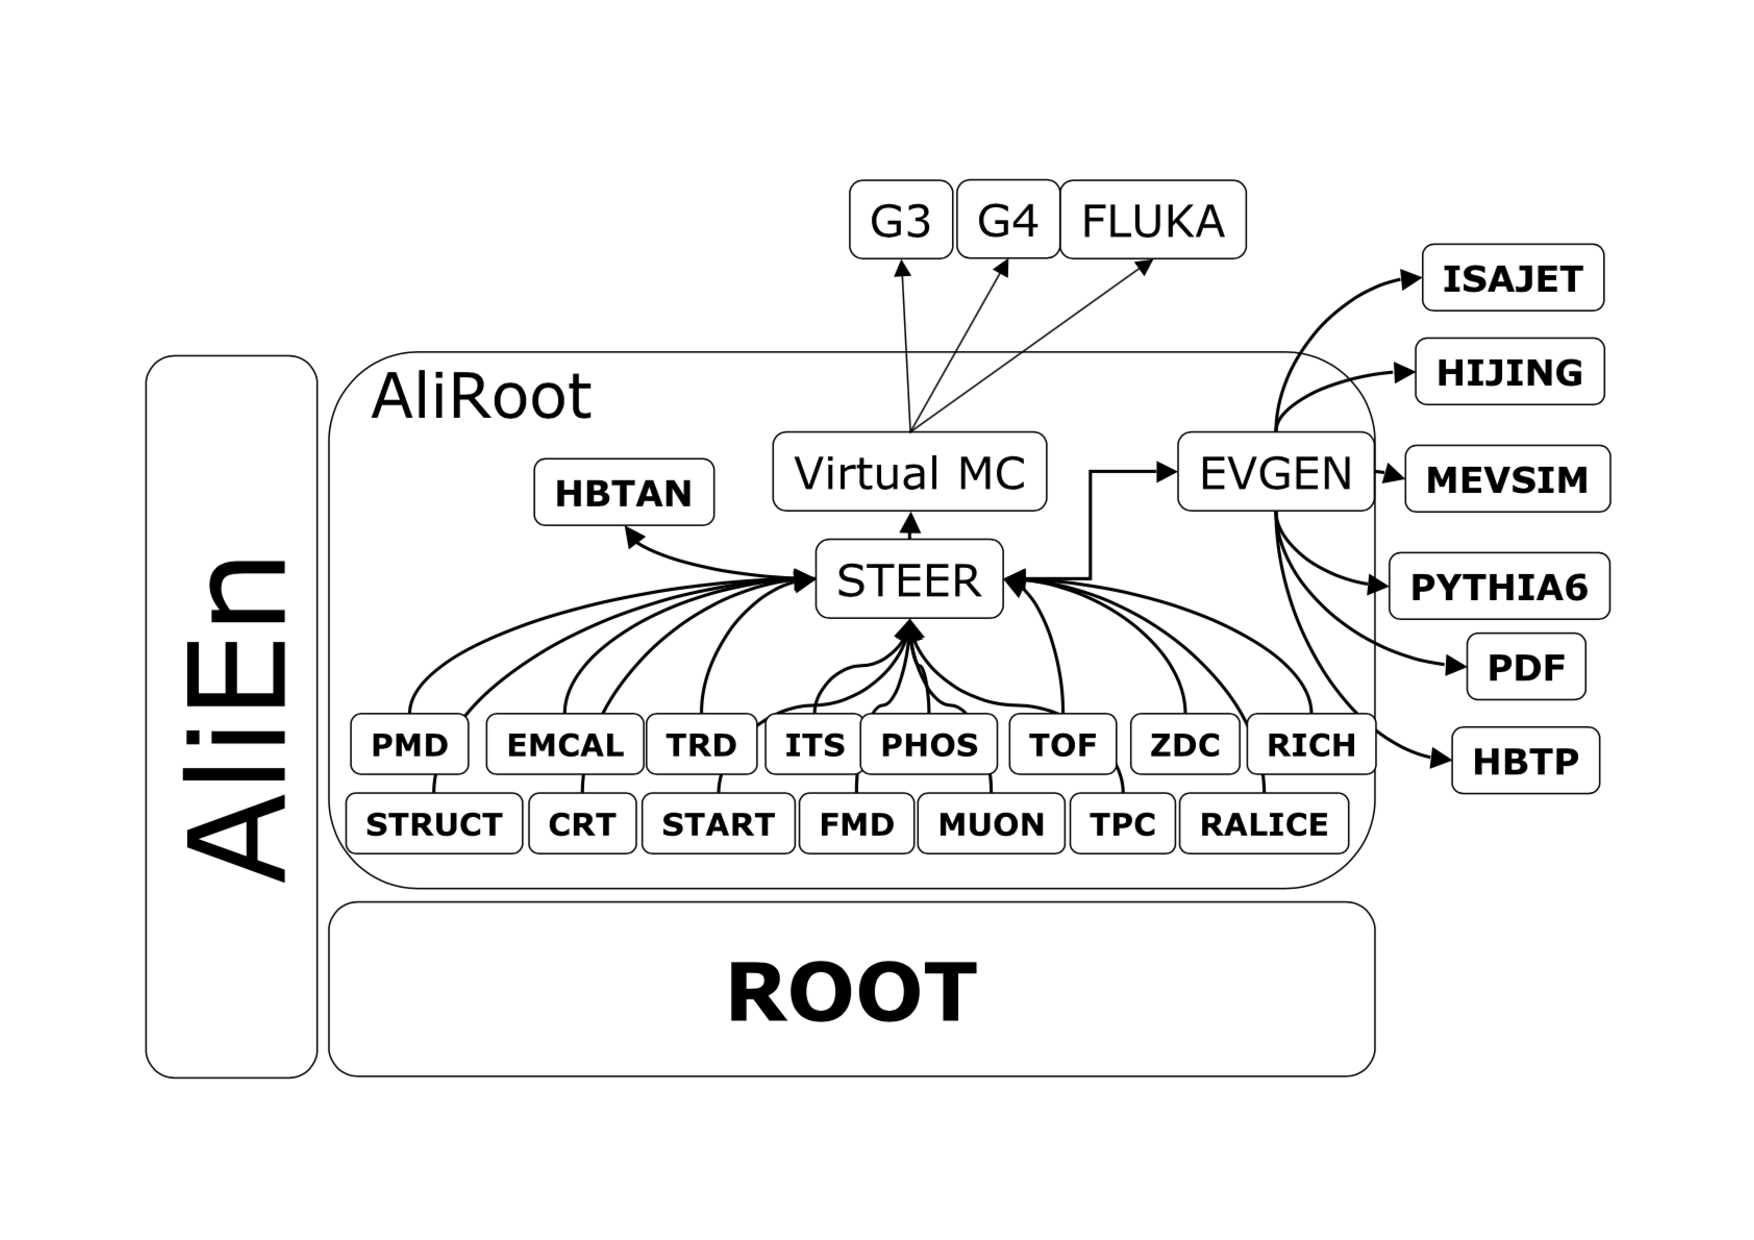
\includegraphics[width=16.cm]{./Version1/FigChapter4/FigureAliRoot}
\caption{Schematic view of the AliRoot framework}
\label{fig:aliroot}
\end{center}
\end{figure}

The central module of the AliRoot framework is STEER (Figure \ref{fig:aliroot}) which provides several common functions such as: steering of program execution for simulation, reconstruction and analysis; general run management, creation and destruction of data structures, initialization and termination of program phases; base classes for simulation, event generation, reconstruction, detectors elements.
For event simulation the framework provides the following functionality:

\newpage
